% TeX root = ./main.tex

% First argument to \section is the title that will go in the table of contents. Second argument is the title that will be printed on the page.
\section[Suites réelles]{Suites réelles}

\subsection{Introduction}

\begin{flushleft}
	\textit{Deux grandeurs inégales étant proposées, si l’on retranche de la plus grande une partie plus grande que sa moitié, si l’on retranche du reste une partie plus grande que sa moitié, et que l’on fait toujours la même chose, il restera une grandeur qui sera plus petite que la plus petite des grandeurs proposées.}
\end{flushleft}
\begin{flushright}
	Euclide
\end{flushright}

\begin{flushleft}
	\textit{Lorsque les valeurs successivement attribuées à une même variable s’approchent indéfiniment d’une valeur finie, de manière à en différer aussi peu qu’on voudra, cette dernière est appelée limite de toutes les autres..}
\end{flushleft}
\begin{flushright}
	Augustin Louis Cauchy
\end{flushright}
Bien avant de faire l’objet d'une étude formalisée, les suites apparaissent dans deux types
de situations : approximations de réels et problèmes de comptages. 


Les problèmes décrits dans les livres de Fibonacci, ou chez les savants arabes qui le
précèdent, se modélisent avec des suites. Oresme calcule des sommes de termes de suites
géométriques au XIVe siècle.


On trouve chez Diophante, puis chez Al-Khwârizmî, des méthodes de résolutions
d’équations du second degré. Le travail novateur d’Al-Khwârizmî reste en partie tributaire de
la tradition (utilisation de considérations géométriques équivalentes à la forme canonique) et
de l'état alors embryonnaire de la notation algébrique, ainsi que de l’absence des nombres
négatifs. Les méthodes actuelles sont un aboutissement de ce long cheminement vers un
formalisme efficace et concis.


Les approximations de réels à l'aide de suites font appel à la notion de limite dont l'appréhension est ancienne. On trouvait en effet déjà cette notion dans des ouvrages d'Euclide. Ce n'est qu'à la moitié du XIXe siècle que la formalisation morderne de la notion de limite est née, grâce au mathématicien Karl Weierstrass.


Ce cours traîtera de généralités sur les suites réelles dans le carde du programe de première.

\subsection{Définitions}

\begin{definition}{Suite réelle}{o}
Une suite réelle est une fonction de $\N$ dans $\R$. On note généralement $(u_n)_{n\in\N}$ un tel objet, mais les notations suivantes sont possibles : $(u_n)_{n\geq 0}$, $(u_n)$ ou simplement $u$.
\end{definition}
\textbf{Vocabulaire :} pour un entier naturel $n$ donné, le \textit{réel} $u_n$ est appelé terme de rang $n$, ou d'indice $n$ de la suite $(u_n)$. On pourra aussi rencontrer l'appellation "terme général".
Les suites peuvent être définies de plusieurs manières différentes. Dans le cadre du programme de 1ère, on retient deux manières principales de définir une suite : 
\begin{itemize}
	\item \textbf{Définition explicite} : Si on possède une fonction $f:\R\to\R$, on peut directement définir une suite en donnant son terme général. Pour tout $n\in\N$, $u_n=f(n)$.
	\item \textbf{Définition par récurrence} : Si on possède une fonction $f:\R\to\R$, on peut définir une suite en donnant deux informations : le premier terme de la suite, en général $u_0$, et comment, pour un entier $n$ donné, le terme $u_{n+1}$ est calculé à partir du terme $u_n$, et ce en donnant une relation de récurrence : pour tout entier naturel $n$, $u_{n+1}=f(u_n)$.
\end{itemize}
\textbf{Remarque :} il n'est pas exclu qu'une suite puisse être définie à partir d'un rang différent de $0$. Dans ce cas là, on note $(u_n)_{n\geq n_0}$, $n_0$ étant l'indice de son premier terme.

\begin{exemple}{Suite définie par récurrence}{o}
Soit une suite $(u_n)$ définie par \[\begin{cases}u_0=1\\ \forall n\in\N,\quad u_{n+1}=2u_n\end{cases}\]
Calculer $u_5$.
\end{exemple}

\begin{exemple}{Suite définie explicitement}{o}
Soit une suite $(u_n)$ définie par \[\forall n\in\N,\quad u_n=n^2+n+1\]
Exprimer $u_{n+1}$.
\end{exemple}

\subsection{Suites arithmétiques et géométriques}
\subsubsection{Suites arithmétiques}
\begin{definition}{Suite arithmétique}{o}
Soit $(u_n)$ une suite réelle. S'il existe un réel $r$ tel que \[\forall n\in\N,\quad u_{n+1}=u_n+r\]
On dit que $(u_n)$ est arithmétique. On appelle $r$ la raison de la suite.
\end{definition}

\begin{exemple}{Suite arithmétique}{o}
La suite $(u_n)$ définie par \[\forall n\in\N,\quad u_n=3n+1\] est arithmétique. Comment le vérifier ?
\end{exemple}

L'exemple précédent amène un point de méthodologie. On se ramène à la définition : le critère qui y est cité est un critère d'existence, il faut montrer l'existence de $r$ vérifiant la relation de récurrence $\forall n\in\N,\ u_{n+1}=u_n+r$. Pour cela, on peut calculer $u_{n+1}-u_n$ pour tout $n$ entier naturel.

\begin{proposition}{Expression explicite d'une suite arithmétique}{o}
Soit $(u_n)$ une suite arithmétique de raison $r\in\R$. On a \[\forall n\in\N,\quad u_n=nr+u_0\]
\end{proposition}

\begin{proof}
	De la définition d'une suite arithmétique, on sait que $\forall n\in\N,\ u_{n+1}-u_n=r$. On peut alors, pour $n\in\N^*$, écrire cette relation $n$ fois comme ceci : 
	\begin{align*}
		u_1-u_0 &= r\\
		u_2-u_1 &= r\\
		\vdots\\
		u_n-u_{n-1} &= r
	\end{align*}
	En sommant toutes les relations, on se rend compte que, d'un côté des égalités, plein de termes s'annulent :
	\begin{align*}
		\cancel{u_1}-u_0 &= r\\
		\cancel{u_2}-\cancel{u_1} &= r\\
		\vdots\\
		u_n-\cancel{u_{n-1}} &= r
	\end{align*}

	Ce qui donne comme résultalt : \[u_n-u_0=\underbrace{r+\dots+r}_{n\text{ fois}}\]
	Comme on somme $n$ égalités, on trouve $n$ fois la raison $r$ à droite, d'où \[u_n-u_0=nr\]
	Et ainsi \[u_n=u_0+nr\]
	Cette relation reste vraie au rang $0$, puisque $u_0=u_0+0\times r$.
\end{proof}

\textbf{Remarque :} de manière réciproque, toute suite $(u_n)_{n\geq 0}$ définie par \[\forall n\in\N,\quad u_n=an+b\] où $a$ et $b$ sont des réels est une suite arithmétique de raison $a$ (et de premier terme $b$).

\begin{exemple}{Expression explicite d'une suite arithmétique}{o}
	Soit $(u_n)$ la suite définie par \[\begin{cases}u_0=1\\\forall n\in\N,\quad u_{n+1}=u_n+3\end{cases}\]
	Donner l'expression du terme général de $(u_n)$.
\end{exemple}
Dans certains contextes, il peut être intéressant de savoir calculer la somme des termes d'une suite. Dans le cas des suites arithmétiques, on sait produire une formule pour la somme des termes, elle découle directement de la somme des $n$ premiers entiers naturels pour un entier $n$ donné.

\begin{lemme}{Somme des premiers entiers naturels}{o}
Soit $n\in\N$. On a \[1+2+\dots+n=\frac{n(n+1)}2\]
\end{lemme}

\begin{proof}
Pour cette démonstration, on utilisera la technique qu'aurait utilisée le petit Gauss (Karl Friedrich Gauss est un mathématicien important du XIXème siècle) pour calculer la somme des entiers entre $1$ et $100$. On écrit la somme dans les deux sens : 
\[
\begin{array}{c c c c c c c}
	1 & + & 2 & + & \dots & + & n\\
	n & + & n-1 & + & \dots & + & 1
\end{array}
\]
On se rend alors compte que pour chaque colonne, la somme des entiers qui s'y trouvent vaut $n+1$ (en effet, $n + 1 = n+1$, $n-1+2=n+1$, $n-2+3=n+1$...). Si on note $S$ la somme $1+2+\dots+n$, on a alors \[2S=\underbrace{(n+1)+\dots+(n+1)}_{n\text{ fois}}\]
Il s'ensuit donc que $2S=n(n+1)$ et donc finalement \[S=\frac{n(n+1)}2\]
\end{proof}

\begin{proposition}{Sommes des termes d'une suite arithmétique}{o}
Soit $(u_n)$ une suite arithmétique de raison $r$ et $n\in\N$. Alors 
\[u_0+u_1+\dots+u_n=(n+1)\frac{u_n+u_0}2\]
\end{proposition}

\begin{proof}
On note $S$ la somme que l'on veut calculer et on écrit
\begin{align*}
	S=u_0+u_1+\dots+u_n &= (0\times r+u_0)+(1\times r+u_0)+\dots+(n\times r+u_0)\\
						&= 0\times r+1\times r+\dots+n\times r+(\underbrace{u_0+\dots+u_0}_{n+1\text{ fois}})\\
						&= r(0+1+\dots+n)+(n+1)u_0
\end{align*}
Ainsi, en utilisant le lemme précédant, on arrive à calculer la somme $1+\dots+n$ et on a 
\[S=r\frac{n(n+1)}2+(n+1)u_0\]
On factorise par $(n+1)$ et on a 
\begin{align*}
	S &= (n+1)\left(u_0+\frac{nr}2\right)\\
	  &= (n+1)\frac{nr+2u_0}2\\
	  &= (n+1)\frac{(nr+u_0)+u_0}2\\
	  &= (n+1)\frac{u_n+u_0}2
\end{align*}
\end{proof}

\subsubsection{Suites géométriques}
\begin{definition}{Suite géométrique}{o}
	Soit $(u_n)$ une suite réelle. S'il existe un réel $q$ tel que \[\forall n\in\N,\quad u_{n+1}=qu_n\]
	alors on dit que $(u_n)$ est géométrique. On appelle $q$ la raison de la suite.
\end{definition}

\begin{exemple}{Suite géométrique}{o}
La suite $(u_n)$ est définie par \[\forall n\in\N,\quad u_n=\frac3{2^n}\]
est géométrique. Comment le vérfier ?
\end{exemple}
Comme pour le cas des suites arithmétiques, l’exemple précédent amène également un point de méthodologie. Il s'agit ici de montrer l’existence de $q$ vérifiant la relation de récurrence $\forall n\in\N u_{n+1} = qu_n$. Pour cela, on peut calculer, après s'être assuré que $u_n$ est non nul pour tout $n$, $\frac{u_{n+1}}{u_n}$ pour tout $n$.


\begin{proposition}{Expression explicite d'une suite géométrique}{o}
	Soit $(u_n)$ une suite géométrique de raison $q\in\R$. On a \[\forall n\in\N,\quad u_n=u_0q^n\]
\end{proposition}

\begin{proof}
	La démonstration est similaire à celle qui a été faite dans le cas des suites arithmétiques. Soit $n\in\N$, on écrit la relation de récurrence $n$ fois comme suit :
	\begin{align*}
		u_1 &= u_0q\\
		u_2 &= u_1q\\
		\vdots\\
		u_n &= u_{n-1}q
	\end{align*}
	En faisant le produit de toutes ces relations, on obtient \[u_1\times\dots\times u_n=u_0q\times\dots\times u_{n-1}q=u_0\times\dots\times u_{n-1}\times q^n\]
	Si $u_0$ et $q$ ne sont pas nuls, aucun des termes de la suite est nul et on peut alors simplifier par $u_1\times\dots\times u_{n-1}$ pour obtenir \[u_n=u_0q^n\]
	Si $u_0$ ou $q$ est nul, la relation reste quand même vraie et c'est une simple vérification.
\end{proof}

\begin{exemple}{Expression explicite d'une suite géométrique}{o}
	Soit $(u_n)$ la suite définie par \[\begin{cases}u_0=3\\\forall n\in\N,\quad u_{n+1}=\frac12u_n\end{cases}\]
	Donner l'expression du terme général de $(u_n)$.
\end{exemple}
Comme pour le cas des suites arithmétiques, on sait donner une expression consise pour la somme des termes d'une suite géométrique. On établit d'abord un premier résultat

\begin{lemme}{Somme des premières puisssance d'un réel différent de $1$}{o}
Soit $q\in\R\backslash\lbrace 1\rbrace$ et $n\in\N$. Alors \[1+q+q^2+\dots+q^n=\frac{1-q^{n+1}}{1-q}\]
\end{lemme}

\begin{proof}
Notons $S=1+q+q^2+\dots+q^n$. Dans ce cas
\[qS=q(1+q+q^2+\dots+q^n)=q+q^2+q^3+\dots+q^{n+1}\]
En effectuant la différence entre $S$ et $qS$, il se produit le même phénomène qu'à la preuve de la proposition 1.3.1, c'est-à-dire un télescopage. Le lecteur se convaincra ainsi que $S-qS=1-q^{n+1}$ et ainsi, comme $1-q\neq 0$ (puisque $q\neq 1$), on a \[S=\frac{1-q^{n+1}}{1-q}\]
\end{proof}

\begin{proposition}{Somme des termes d'une suite géométrique}{o}
	Soit $(u_n)$ une suite géométrique de raison $q\in\R$. Soit $n\in\N$, alors \[u_0+u_1+\dots+u_n=u_0\frac{1-q^{n+1}}{1-q}\]
\end{proposition}

\begin{proof}
	En écrivant la somme, on se rend compte qu'il est possible de factoriser par $u_0$, sachant l'expression explicite de $(u_n)$ 
	\begin{align*}
		u_0+u_1+\dots+u_n &= u_0+u_0q+\dots+u_0q^n\\
						  &= u_0(1+q+\dots+q^n)
	\end{align*}
	On utilise le lemme précédant pour établir que \[u_0+u_1+\dots+u_n=u_0\frac{1-q^{n+1}}{1-q}\]
\end{proof}

\subsection{Sens de variations d'une suite}
\subsubsection{Suites monotones et constantes}

\begin{definition}{Sens de variations}{o}
	Soit $(u_n)$ une suite réelle. 
	\begin{itemize}
		\item Si $\forall n\in\N,\ u_{n+1}\geq u_n$, on dit que la suite est \textbf{croissante}.
		\item Si $\forall n\in\N,\ u_{n+1}\leq u_n$, on dit que la suite est \textbf{décroissante}.
		\item S'il existe un réel $a$ tel que $\forall n\in\N,\ u_n=a$, on dit que la suite est \textbf{constante}.
		On dit que $(u_n)$ est \textbf{monotone} si elle est croissante ou décroissante.  
	\end{itemize}
\end{definition}
\textbf{Remarque :} il existe un autre vocabulaire pour les suites \textit{presque} constantes. En effet, s'il existe un réel $a$ et un entier $n_0$ tel que $\forall n\geq n_0,\ u_n=a$, alors on dit que $(u_n)$ est \textbf{stationnaire}.


\textbf{Remarque :} on parle de stricte croissance (ou stricte décroissance) lorsque les inégalités ci-dessus sont strictes.
\begin{exemple}{Cette suite est-elle monotone ?}{o}
	Soit $(u_n)$ une suite définie par \[\begin{cases} u_0=0\\\forall n\in\N,\quad u_{n+1}=u_n+(1-n)^2\end{cases}\]
	Déterminer si cette suite est monotone. Si oui, donner sa monotonie (dire si elle est croissante ou décroissante).
\end{exemple}

\textbf{Remarque : } Si une suite $(u_n)$ est à termes strictement positifs, une autre manière de déterminer son sens de variation est de calculer, pour tout $n\in\N$ le quotient $\frac{u_{n+1}}{u_n}$. Trois cas se présentent :

\begin{itemize}
	\item $\forall n\in\N,\ \frac{u_{n+1}}{u_n} \leq 1$ et dans ce cas la suite est décroissante.
	\item $\forall n\in\N,\ \frac{u_{n+1}}{u_n} = 1$ et dans ce cas la suite est constante.
	\item $\forall n\in\N,\ \frac{u_{n+1}}{u_n} \geq 1$ et dans ce cas la suite est croissante.
\end{itemize}

\subsubsection{Cas des suites arithmétiques et géométriques}

\begin{proposition}{Sens de variation des suites arithmétiques}{o}
Soit $(u_n)$ une suite arithmétique de raison $r\in\R$. Ainsi 
\begin{itemize}
	\item Si $r\geq 0$, alors $(u_n)$ est croissante.
	\item Si $r\leq 0$, alors $(u_n)$ est décroissante.
\end{itemize}
\end{proposition}
\begin{proof}
Soit $n\in\N$, on sait que $u_{n+1}=u_n+r$, donc $u_{n+1}-u_n=r$. Ainsi, si $r\leq 0$ $(u_n)$ est décroissante et si $r\geq 0$ $(u_n)$ est croissante d'après les définitions.
\end{proof}

\begin{proposition}{Sens de variation des suites géométriques}{o}
Soit $(u_n)$ une suite géométrique de raison $q\in\R$. Plusieurs cas se présentent : 
\begin{itemize}
	\item Si $q > 0$, alors, si $u_0$ est positif (resp. négatif) 
	\begin{itemize}
		\item Si $q \geq 1$, alors $(u_n)$ est croissante (resp. décroissante).
		\item Si $q = 1$, alors $(u_n)$ est constante.
		\item Si $q \leq 1$, alors $(u_n)$ est décroissante (resp. croissante).
	\end{itemize}
	\item Si $q = 0$, alors $(u_n)$ est stationnaire égale à $0$ à partir du rang $1$.
	\item Si $q < 0$, on ne peut malheureusement rien dire...
\end{itemize}
\end{proposition}

\begin{exemple}{Sens de variation de suites arithmétiques et géométriques}{o}
	Soit $(u_n)$ la suite définie par \[\begin{cases}u_0=-2\\ \forall n\in\N,\quad u_{n+1}=\frac12 u_n\end{cases}\]
	Que dire de son sens de variation ? Donner un exemple d'une suite arithmétique décroissante. 
\end{exemple}

\subsubsection{Cas des suites définies explicitement}
Au tout début de ce chapitre sur les suites réelles, deux manières de définir une suite ont été évoquées; l'une d'entre elles est la définition explicite. Dans cette définition, la fonction $f:\R\to\R$ dont il était question peut être appelée fonction associée.
\begin{proposition}{Montonie d'une suite que l'on peut exprimer explicitement}{o}
	Soit $(u_n)_{n\geq n_0}$ une suite réelle dont on sait exprimer le terme général. Si la fonction associée à $(u_n)$ est monotone sur $[n_0,+\infty[$, alors la suite $(u_n)$ est également monotone de même monotonie que sa fonction associée.
\end{proposition}

\begin{exemple}{Un exemple qui nous fait faire des révisions}{o}
	Déterminer la monotonie des suites définies par les termes généraux suivants
	\begin{enumerate}
		\begin{minipage}{0.4\linewidth}
		    \item $u_n=n^2$
		\end{minipage}
		\begin{minipage}{0.4\linewidth}
		    \item $u_n=\sqrt{n}$
		\end{minipage}
		\begin{minipage}{0.4\linewidth}
		    \item $u_n=\frac1n$
		\end{minipage}
	\end{enumerate}
\end{exemple}

\subsection{Représentation graphique d'une suite}
Une suite est représentée graphiquement à l'aide de points ou de symboles positionnés aux images par $u$ des entiers naturels plus grand que $n_0$ (l'indice du premier terme de la suite).
\begin{center}
	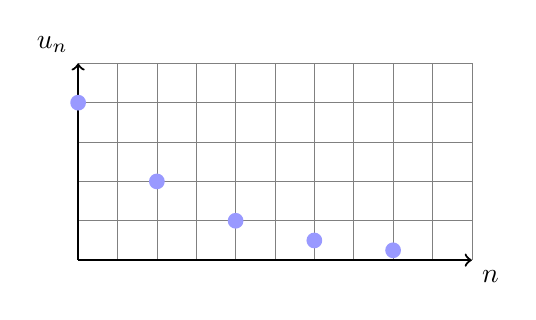
\begin{tikzpicture}
		\draw[step=0.5, gray, very thin] (0,0) grid (5,2.5);
		\draw[->, thick] (0,0) -- (0,2.5) node [above left] {$u_n$};
		\draw[->, thick] (0,0) -- (5,0) node [below right] {$n$};
		\fill[blue!40] (0,2) circle (0.1);
		\fill[blue!40] (1,1) circle (0.1);
		\fill[blue!40] (2,0.5) circle (0.1);
		\fill[blue!40] (3,0.25) circle (0.1);
		\fill[blue!40] (4,0.125) circle (0.1);
	\end{tikzpicture}
\end{center}
Ci-dessus, un exemple de la suite $(u_n)$ définie par $\forall n\in\N,\ u_n=\frac1{2^n}$.
\begin{exemple}{Représente-moi ça}{o}
Représentés graphiquement les suites de l'exemple 1.4.3.
\end{exemple}

\subsection{Limite d'une suite}
Dans le cadre du programme de première, aucune définition ou formalisation de la notion de limite n'est à connaître; dans cette partie, il s'agira ainsi seulement de comprendre intuitivement à quoi cela correspond. 

\subsubsection{Limite finie}
Soit $(u_n)$ la suite définie par \[\forall n\in\N,\quad u_n=\frac1{2^n}+1\]
On représente les premiers termes de la suite graphiquement : 

\begin{center}
	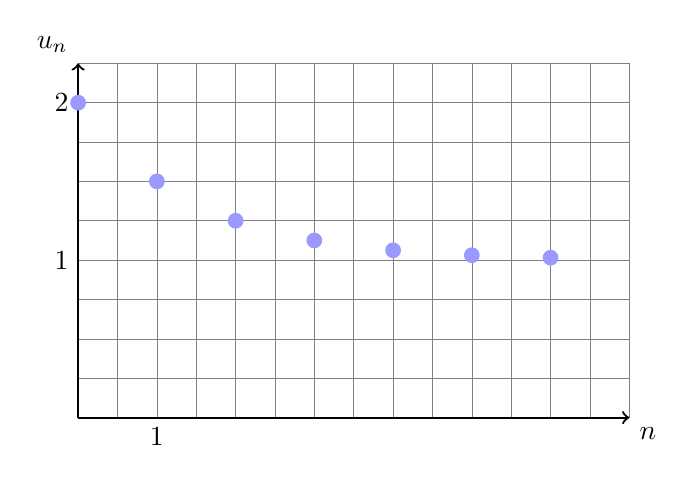
\begin{tikzpicture}
		\draw[step=0.5, gray, very thin] (0,0) grid (7,4.5);
		\draw[->, thick] (0,0) -- (0,4.5) node [above left] {$u_n$};
		\draw[->, thick] (0,0) -- (7,0) node [below right] {$n$};
		\node at (0, 2) [left] {$1$};
		\node at (0, 4) [left] {$2$};
		\node at (1, 0) [below] {$1$};
		\fill[blue!40] (0,4) circle (0.1);
		\fill[blue!40] (1,3) circle (0.1);
		\fill[blue!40] (2,2.5) circle (0.1);
		\fill[blue!40] (3,2.25) circle (0.1);
		\fill[blue!40] (4,2.125) circle (0.1);
		\fill[blue!40] (5,2.0625) circle (0.1);
		\fill[blue!40] (6,2.03125) circle (0.1);
	\end{tikzpicture}
\end{center}

Visuellement, on peut déjà remarquer que les termes de la suite, représenter par les points bleus, se raprochent d'autant plus que $n$ est grand d'une certaine valeur, ici 1. On est ici en présence d'une suite qui possède une limite \textit{finie} égale à 1. En réalité, on dit qu'un réel est limite d'une suite si, peu importe la distance $\delta$ que l'on choisit, aussi petite soit-elle, pourvu qu'elle ne soit pas nulle, il existe un rang $n_0$ à partir duquel tous les termes de la suite se trouve à une distance plus petite que $\delta$ du candidat limite. Graphiquement, on peut représenter le choix de cette distance $\delta$ avec un \textit{tube} de largeur $2\delta$ :

\begin{center}
	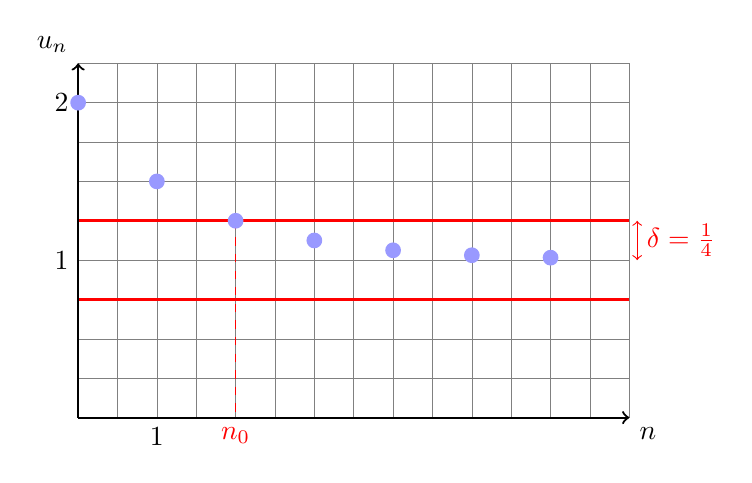
\begin{tikzpicture}
		\draw[step=0.5, gray, very thin] (0,0) grid (7,4.5);
		\draw[red, very thick] (0,2.5) -- (7,2.5);
		\draw[red, very thick] (0,1.5) -- (7,1.5);
		\draw[dashed, red] (2,2.5) -- (2,0);
		\draw[red, <->] (7.1,2.5) -- (7.1,2) node [midway, right] {\color{red} $\delta = \frac14$};
		\node at (2, 0) [below] {\color{red}$n_0$};
		\draw[->, thick] (0,0) -- (0,4.5) node [above left] {$u_n$};
		\draw[->, thick] (0,0) -- (7,0) node [below right] {$n$};
		\node at (0, 2) [left] {$1$};
		\node at (0, 4) [left] {$2$};
		\node at (1, 0) [below] {$1$};
		\fill[blue!40] (0,4) circle (0.1);
		\fill[blue!40] (1,3) circle (0.1);
		\fill[blue!40] (2,2.5) circle (0.1);
		\fill[blue!40] (3,2.25) circle (0.1);
		\fill[blue!40] (4,2.125) circle (0.1);
		\fill[blue!40] (5,2.0625) circle (0.1);
		\fill[blue!40] (6,2.03125) circle (0.1);
	\end{tikzpicture}
\end{center}

\begin{exemple}{Trouver $n_0$}{o}
	Soit $(u_n)$ la suite définie par \[\forall n\in\N,\quad u_n=\frac{2n+1}{3n-3}\]
	Représenter graphiquer les premiers termes de cette suite. En sachant que $u$ possède une limite finie égale à $\frac23$, déterminer graphiquement le rang à partir duquel tous les termes de la suite sont à une distance inférieure à $\delta=\frac12$ de la limite. 
\end{exemple}

\subsubsection{Limite Infinie}
La définition pour ce type de limites est similaire à celui que l'on a vu précédemment, à la seule différence que, au lieu de choisir un tube, on choisit un seuil. On dit qu'une suite $(u_n)$ a pour limite $+\infty$ (resp. $-\infty$) si pour tout réel $A$ il existe un rang $n_0$ à partir duquel tous les termes de la suite sont supérieurs à (resp. inférieurs à) $A$.

Graphiquement, on peut représenter le choix du réel $A$ par une simple \textit{barre} horizontale :
\begin{center}
	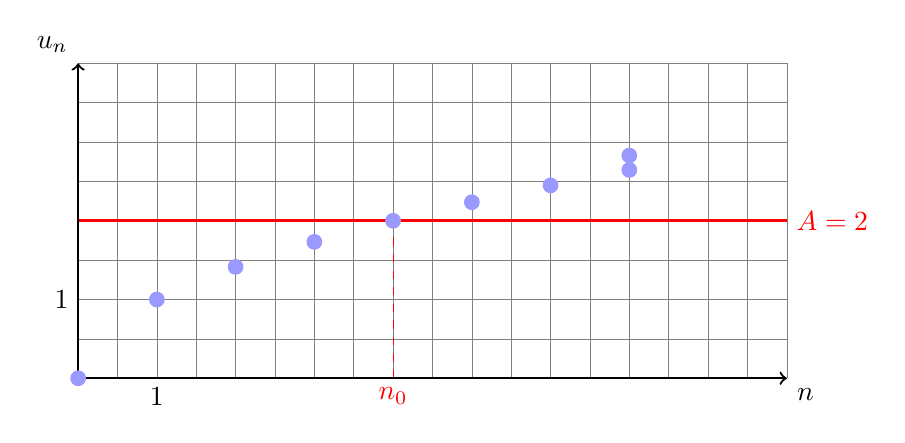
\begin{tikzpicture}
		\draw[step=0.5, gray, very thin] (0,0) grid (9,4);
		\draw[red, very thick] (0,2) -- (9,2);
		\node at (9,2) [right] {\color{red}$A=2$};
		\draw[dashed, red] (4, 2) -- (4,0);
		\node at (4, 0) [below] {\color{red}$n_0$};
		\draw[->, thick] (0,0) -- (0,4) node [above left] {$u_n$};
		\draw[->, thick] (0,0) -- (9,0) node [below right] {$n$};
		\node at (0, 1) [left] {$1$};
		\node at (1, 0) [below] {$1$};
		\fill[blue!40] (0,0) circle (0.1);
		\fill[blue!40] (1,1) circle (0.1);
		\fill[blue!40] (2,1.4142135623730951) circle (0.1);
		\fill[blue!40] (3,1.7320508075688772) circle (0.1);
		\fill[blue!40] (4,2) circle (0.1);
		\fill[blue!40] (5,2.23606797749979) circle (0.1);
		\fill[blue!40] (6,2.449489742783178) circle (0.1);
		\fill[blue!40] (7,2.6457513110645907) circle (0.1);
		\fill[blue!40] (7,2.8284271247461903) circle (0.1);
	\end{tikzpicture}
\end{center}
La suite représentée ci-dessus a pour terme général $u_n=\sqrt n$.

\newpage
\section[Polynômes du second degré]{Polynômes du second degré}

\subsection{Généralités}
\begin{definition}{Fonction polynomiale de degré 2}{o}
On appelle fonction polynômiale de degré 2 toute fonction définie sur $\R$ pouvant s'écrire sous la forme $P(x)=ax^2+bx+c$ où $a,b$ et $c$ sont trois réels avec $a\neq 0$.
\end{definition}
\textbf{Vocabulaire :} les trois réels $a,b$ et $c$ sont appelés coefficients de $P$ et $a$ est appelé le coefficient dominant. 


\textbf{Remarque : } même si il existe une différence entre les objets mathématiques appelés "polynôme" et "fonction polynômiale", on se permet dans la suite de confondre fonction polynomiale du second degré et polynôme de degré 2. 

\begin{definition}{Racine d'un polynôme de degré 2}{o}
	Soit $P$ un polynôme de degré $2$ et $\alpha\in\R$. Si $P(\alpha)=0$, alors on dit que $\alpha$ est racine de $P$.
\end{definition}
\textbf{Remarque : } les racines n'existent pas toujours. 
\begin{proposition}{Nombre de racines d'un polynôme de degré deux}{o}
	Soit $P$ un polynôme de degré $2$. $P$ admet au plus $2$ racines.
\end{proposition}

\begin{proposition}{Coefficients de deux polynômes égaux}{o}
	Deux polynômes de degré deux égaux ont mêmes coefficients.
\end{proposition}

\subsection{Forme canonique et forme factorisée}
Il existe plusieurs expressions algébriques pour un polynomiale. L'une des capacités attendues des élèves dans ce chapitre c'est de savoir choisir la bonne forme à utiliser dans le cadre d'un exercice ou de la résolution d'un problème. Mais bien sûr, avant, il faut les connaître ! La forme vue dans la partie précédent et qui a servi à définir l'objet que l'on étudie ici s'appelle \textit{forme développée} du polynôme. 

\begin{proposition}{Forme canonique d'un polynôme de degré $2$}{o}
Soit $P$ un polynôme de degré $2$ de forme développée $P(x)=ax^2+bx+c$ où $a,b$ et $c$ sont trois réels avec $a\neq 0$. Alors, pour tout réel $x$, on a 
\[P(x)=a\left[\left(x+\frac b{2a}\right)^2-\frac{b^2-4ac}{4a^2}\right]\]
\end{proposition}

\begin{proof}
	Soit $x$ un réel, on a 
	\begin{align*}
		P(x) &= ax^2+bx+c\\
			 &= a\left(x^2+\frac bax+\frac ca\right)\\
			 &= a\Big(\underbrace{x^2+2\frac b{2a}x}_{=\left(x+\frac b{2a}\right)^2-\left(\frac b{2a}\right)^2}+\frac ca\Big)\\
			 &= a\left[\left(x+\frac b{2a}\right)^2-\frac{b^2}{4a^2}+\frac ca\right]\\
			 &= a\left[\left(x+\frac b{2a}\right)^2-\frac{b^2-4ac}{4a^2}\right]
	\end{align*}
\end{proof}

\begin{proposition}{Forme factorisée d'un polynôme de degré $2$}{o}
	Soit $P$ un polynôme de degré $2$ de coefficient dominant $a\neq 0$. Si $P$ admet deux racines $\alpha$ et $\beta$ disctinctes ou confondues (cela veut dire qu'il est possible d'avoir $\alpha=\beta$), alors on peut écrire \[P(x)=a(x-\alpha)(x-\beta)\]
\end{proposition}

\subsection{Équations du second degré et signe d'une fonction polynomiale de degré $2$}

\subsection{Compléments}

